\chapter{General Addenda}
\section{Qualitative Benchmark results}
\begin{figure}[H]
\centering
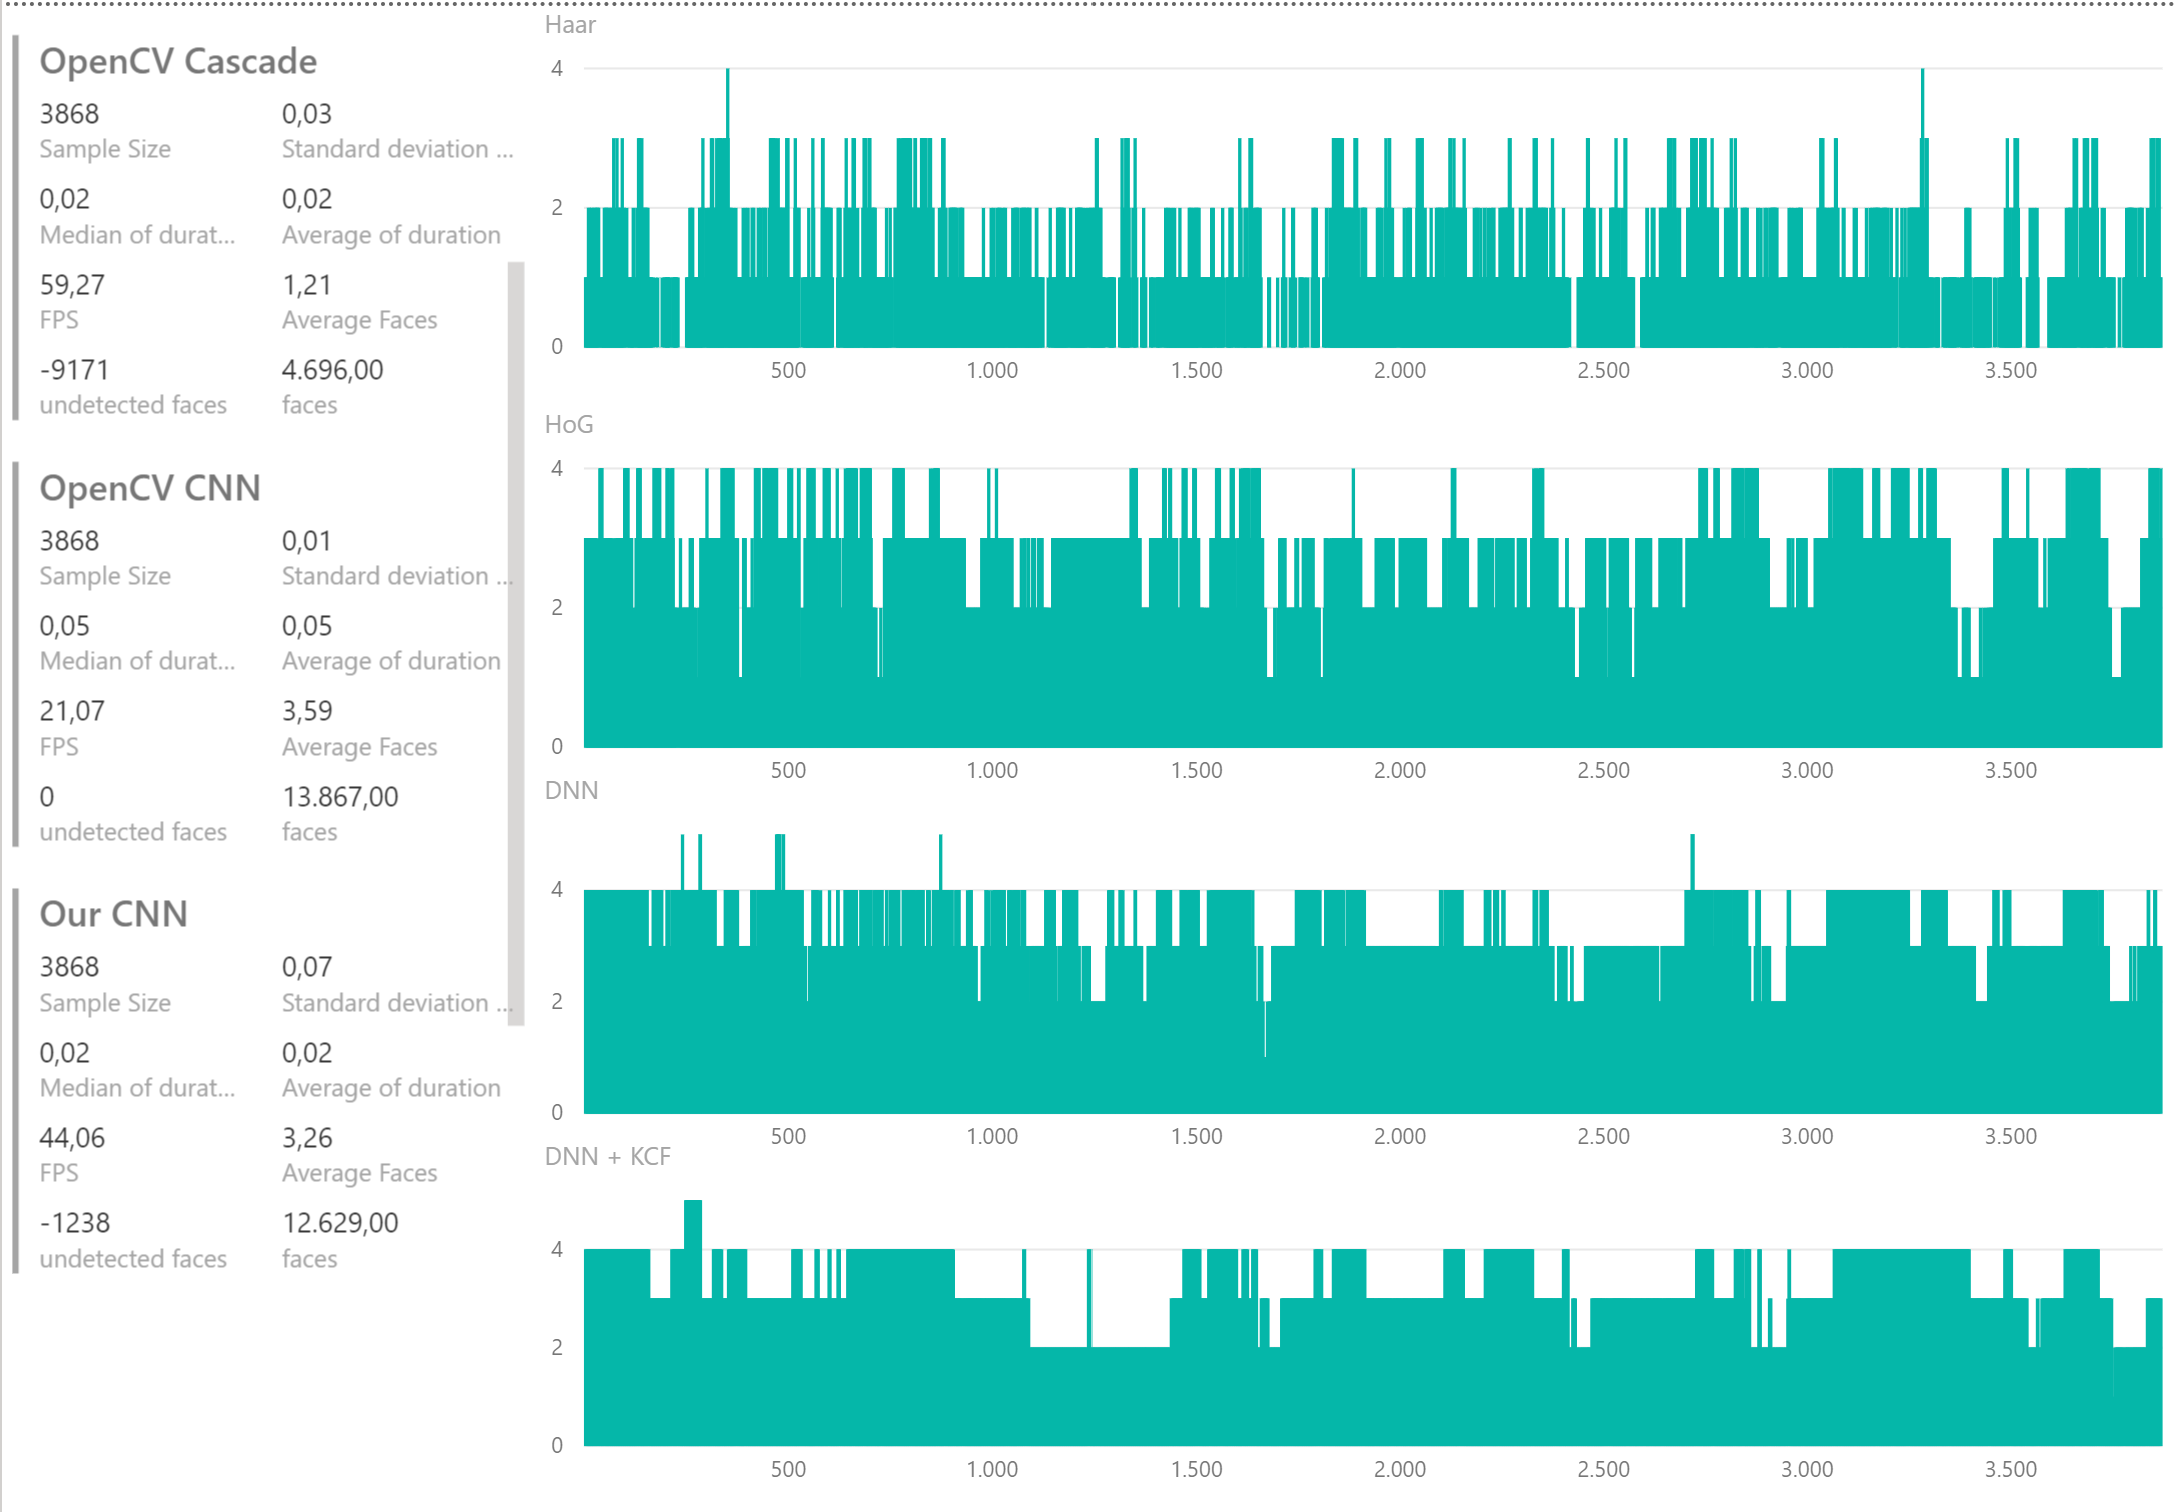
\includegraphics[width=\columnwidth]{media/qualitativebenchmark.png}
\caption{Analytics Dashboard for qualitative benchmark results}
\label{fig:pbidashboard}
\end{figure}

\section{Initial Assessment of Approaches (Notes)}
\subsection{Motion Detection Approach}
\begin{itemize}
    \item The system would have a ‘start-up phase’ where all faces visible at that moment in the car will be detected (using a very accurate face detection method (doesn’t have to be in real time, one second delay is acceptable)
    \item After the ‘start-up phase’ which will last approximately one second all detected faces are evaluated and facial landmarks are calculated using HoG (HoG only created for the local face region to save resources)
    \item During runtime, the system will no longer run face detection on the entire feed, instead existing faces will be tracked using a KLT feature tracker.
    \item During runtime, a motion detection algorithm will detect areas in the feed that change
    \item When change is detected the algorithm triggers a \gls{cnn} or HoG/SVM that will then try to detect a face in the limited area of change.
    \item If no change is detected the face detection system won’t be triggered
    \item Since the camera will be mounted in a fixed position a motion detection approach seems to be the best way to implement the system
    \item Benefits:
        \begin{itemize}
        \item If implemented correctly the approach should run in real time
        \item As long as there is little change in the feed, the system can track faces extremely efficiently (usually in a car there is little change, people don’t enter/exit cars every minute)
        \end{itemize}
    \item Challenges:
            \begin{itemize}
        \item System can be tricked if someone moves his face extremely slowly into the feed
        \item System works for the specified case (mounted camera in a car), however it is not able to deal with an input feed that changes a lot
        \item Bridging the gap between startup evaluation and runtime face tracking
        \item Complex implementation
                \end{itemize}
\end{itemize}
\subsection{Face Detection Approach (CNN)}
\begin{itemize}
    \item The system designed would detect faces using a \gls{cnn} that would run on the GPU of the Raspberry PI. Since the PI doesn’t have the computational power to fully evaluate the video feed in real time some optimizations need to be performed. 
    \item A solution would be to reduce the resolution of the feed significantly and train a model that is able to detect face like structures (schematic structures, no details). 
    \item After detecting those structures, a local HoG needs to be computed to detect facial landmarks and verify that the object is a face. 
    \item As soon as a face has been detected, the area of the face is no longer processed by the face detection algorithm to save resources. However the system still needs to be able to follow movements etc.. We can fulfill that constraint by using a feature tracker like KLT.
    \item Benefits:
            \begin{itemize}
        \item Most accurate implementation
        \item CNN runs well on GPU
                \end{itemize}
    \item Challenges:
            \begin{itemize}
        \item Probably won’t fulfill resource constraints
        \item Single components might need to be replaced by faster/less accurate ones
        \item Complex implementation and model training
                \end{itemize}
\end{itemize}
\subsection{Face Detection Approach (HoG \& Linear SVM)}
\begin{itemize}
    \item Detect multiple faces in real time using HoG \& a linear SVM
    \item Will probably not run in real time so the only option would be to combine it with the previous approaches 
    \item Benefits:
            \begin{itemize}
        \item Fast on CPU
                \end{itemize}
    \item Challenges:
            \begin{itemize}
        \item Without additional optimizations the system will not run in real time
                \end{itemize}
\end{itemize}
\subsection{Face Detection Approach (Viola Jones Algorithm)}
\begin{itemize}
    \item Detecting multiple faces in real time using the Viola Jones Algorithm
    \item Haar Cascade -> Integral Image -> Adaboost -> Cascading Classifiers
    \item Benefits:
            \begin{itemize}
        \item Easy to implement
        \item Performance
                \end{itemize}
    \item Challenges:
            \begin{itemize}
        \item Low accuracy, probably won’t be fast enough
        \item Performs wore in almost every area compared to (HoG + Linear SVM)
                \end{itemize}
\end{itemize}